\chapter{Sequence prediction for running cases}
\label{chap:taking-inspiration}
While a number of works have demonstrated the applicability of LSTM neural networks to Predictive Process Monitoring, most have left out a perspective on the sequence prediction problem from Natural Language Processing (NLP). In this chapter we outline how we take inspiration from sequence prediction in NLP, and thus add to improvement area 3 from \autoref{sec:intro:contribution}.

We establish the connection between processes and sequences by connecting their definitions in \autoref{sec:contrib:case-sequence-understanding}. This provides the underpinning for introducing two NLP-inspired approaches for predicting the next activity in a case. These are presented in \autoref{sec:contrib:sp2-inspiration} and \autoref{sec:contrib:pfs-inspiration}.

\section{Understanding a trace as a sequence}\label{sec:contrib:case-sequence-understanding}
The definition for sequences presented in \autoref{sec:background:sequence-prediction} and the definition of traces in \autoref{sec:log-structure} will be connected in this section to make it clear how events can be understood as itemsets.

Both a trace $\#_{trace}(c)$ from a case $c$ and a sequence $seq$ are already defined in a very similar manner:
\begin{equation*}
\begin{split}
seq           &=  \langle s_1,s_2\cdots s_l \rangle\ |\ \forall\ 0 \leq j \leq l: s_j \subseteq \mathscr{I}\\
\#_{trace}(c) &= \langle e_1, e_2, e_3 \dots, e_n \rangle
\end{split}
\end{equation*}

Any itemset consists of items $s = (i_1, i_2 \cdots i_n)$ with $i \in \mathscr{I}$. Events are made up of attributes that are accessed via the $\#$ operator.
In a first step, attributes are defined as items, so that any possible value from any attribute can be understood as an item:

$$\mathscr{I} = \{\#_{a}(e)\ |\ c \in L\wedge e \in \#_{trace}(c) \wedge a \in attrs(e)\}$$

In a second step, a schema is applied to the itemsets. Without it, the itemset that should represent an event could consist e.g. only out of timestamps, as $s \subseteq \mathscr{I}$ does not place any restrictions on the content of $s$.
The schema also provides the tabular format required for machine learning applications, and is introduced as a direct mapping from event $e$ to itemset $s$:

$$ s = (i_1, i_2 \cdots i_n)\ |\ i_i = \#_{attrs(e)[i]}(e) $$

The definition places each item on a specific place in the itemset, depending on the index in the attribute list $attr(e)$. Still, the original condition $s \subseteq \mathscr{I}$ hold true, and now permits sequence prediction on traces.

\section{Adapting a competition submission}\label{sec:contrib:sp2-inspiration}
Shibata et al.'s bipartite network architecture has shown outstanding performance in the SPiCe competition~\cite{web:spice}. Under the assumption that a case exhibits properties similar to sentences, we adapt it for use in the business process domain.

\autoref{fig:sp2-architecture} displays how the original network architecture from Shibata et al. was adapted. The word embedding layers were removed on the sequence data input and replaced with a fully-connected Dense layer on the right. Furthermore, the hidden layer dimensions were adapted following the example by Schönig et al.~\cite{schoenig2018}. The model will be trained on whole events and SP-2 features, whereas the latter is fed in on the right input layer. This approach will be referred to as SP2 in the following.\\

The model uses $n$ units on the first input layer, denoting the dimensionality of the input vector with its encoded activity name, timestamps and other event attributes. It puts out the next activity in one-hot encoded form through $m$ units, thus modelling the task as a multi-classification problem.

In contrast to Evermann et al. and Shibata et al., the number of units $m+n$ in the hidden layers is a function of the input unit count and the output unit count. This follows general advice not to introduce bottlenecks in the hidden layers by using fewer units than required in the output layer. Furthermore, dropout layers have been introduced to prevent overfitting. Another contrast to Shibata et al. is the removal of the embedding layers above the inputs. We opted for this strategy since the dimensionality of activity names is typically a lot lower than it would be for words in a sentence.

The SP-2 features are fed in higher up on the right side of the tree, passing through a ReLU-activated, fully-connected layer, before concatenation with the LSTM output. Finally, the concatenated vectors are processed by fully-connected layers, with the commonly used Softmax activation function producing the classification.

\begin{figure}[ht]
    \centering
    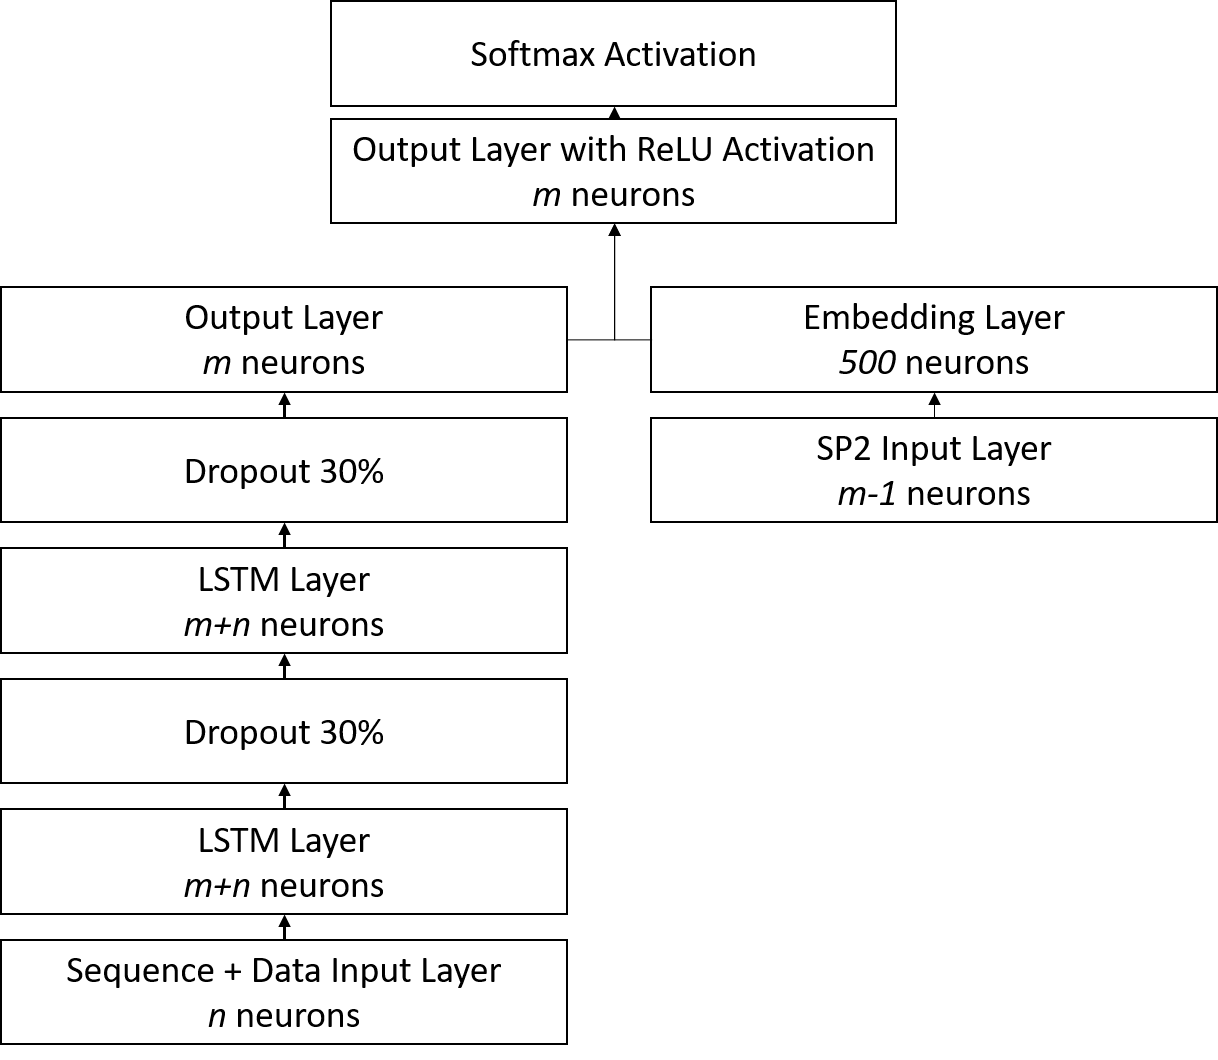
\includegraphics[width=0.8\textwidth]{gfx/sp2-network-architecture.png}
    \caption{SP2 network architecture and its dimensions}
    \label{fig:sp2-architecture}
\end{figure}

\section{Encoding subsequence occurrence}
\label{sec:contrib:pfs-inspiration}
Klinkmüller et al.~\cite{klinkmuller2018reliablemonitoring} compared different feature representations and found that sub-trace occurence features help the model cover a broader variety of relationships. While they found this to be true for random forests, we want to investigate the applicability of such features for LSTM neural networks since we established the similarity of traces and sequences. While the results from Francescomarino et al. are discouraging~\cite{francescomarino2017}, another network architecture can make a difference. As SP-2 features already encode history and subsequence encodings do the same on a higher level of abstraction, we take the SP2 model architecture and inject different features in place of the SP-2 features. Said features and the corresponding architecture will henceforth be referred to as PFS, as illustrated in \autoref{fig:pfs-architecture}. The acronym PFS originates from the word PrefixSpan, which is the name of the algorithm used in \autoref{chap:evaluation} to mine the subsequences.

\begin{figure}[ht]
    \centering
    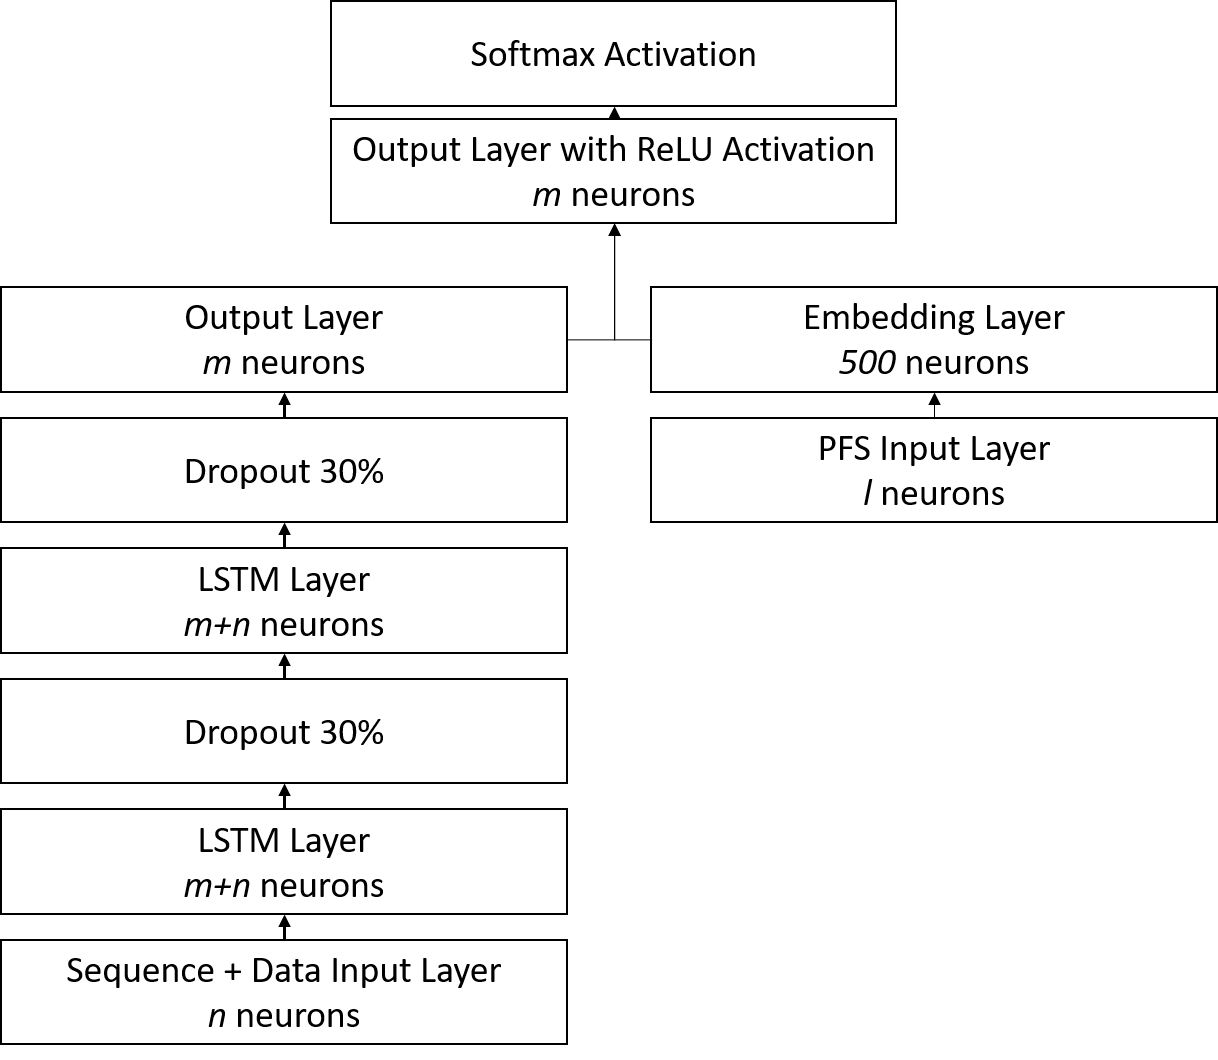
\includegraphics[width=0.8\textwidth]{gfx/pfs-network-architecture.png}
    \caption{PFS network architecture and its dimensions}
    \label{fig:pfs-architecture}
\end{figure}
